%!TEX root = main.tex
\section{Implementación} 
Para realizar la aplicación de la teoría anteriormente explicada, utilizamos Google Colab y Python, junto con las librerías \texttt{unireedsolomon}, \texttt{biopython}, \texttt{matplotlib}, \texttt{py3Dmol} y \texttt{nglview}.\\
Inicialmente para dar un contexto de las estructuras que estamos utilizando, através de \texttt{py3Dmol} y \texttt{nglview} mostramos el modelo de ADN.Posteriormente, utilizando la librería \texttt{biopython}, para una cadena de ADN, mostramos cuál sería su cadena complementaria y la inversa de esta. Esto nos permite ilustrar cómo estas cadenas están anidadas entre sí. Esta aplicación la hicimos através del siguiente código 

\begin{lstlisting}[language=Python]
from Bio.Seq import Seq 
from Bio.SeqUtils import gc_fraction

# Aqui poner la cadena que quieran
cadena_adn = Seq("AGCTAGCTAGCTAAGCTGTA")

# cadena complementaria
cadena_complementaria = cadena_adn.complement()

# inversa complementaria o cadena opuesta
cadena_inversa_complementaria = cadena_adn.reverse_complement()

print("Cadena ADN: ", cadena_adn)
print("Cadena complementaria: ", cadena_complementaria)
print("Cadena inversa complementaria: ", cadena_inversa_complementaria)
\end{lstlisting}
lo cual se puede ilustrar de la siguiente manera
\begin{figure}[h]
\centering
        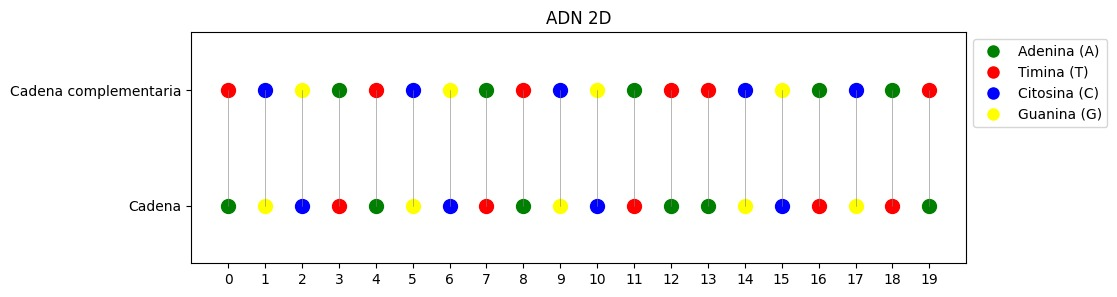
\includegraphics[scale=0.25]{adn1.jpeg} 
    \end{figure}

Aunque no utilizaremos este proceso en los siguientes pasos, mostramos cómo se realiza la transcripción de ADN a ARN y cómo se traduce el ARN a proteínas.

\begin{lstlisting}[language=Python]
arn = cadena_adn.transcribe()
print(f"Secuencia ARN: {arn}")

proteina = arn.translate()
print(f"Proteina: {proteina}")
\end{lstlisting}
Ilustrando un poco como se realiza la transcripción de ADN a ARN hicimos el siguiente gráfico
\begin{figure}[h]
\centering
        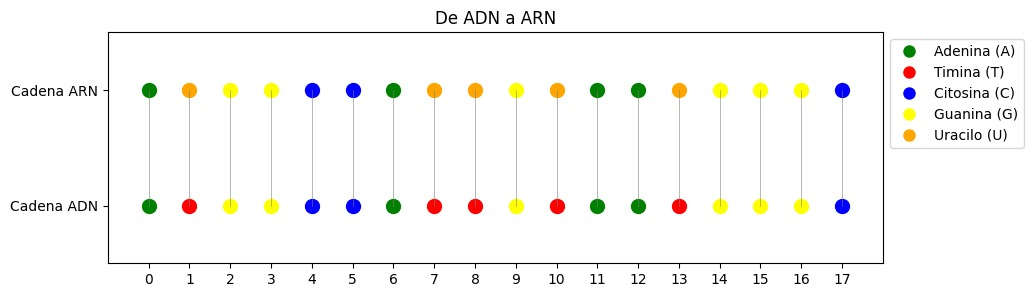
\includegraphics[scale=0.25]{arn.png} 
    \end{figure}
Utilizando todas las librerias anteriormente mencionadas realizamos la representación gráfica de la proteina a la que se puede transcribir la cadena de ARN (estas imágenes puede verlas en el archivo de código).\\

\subsection{Ejemplo corrección de Errores con Hamming(7,4)}

En este ejemplo vamos a partir de una cadena de ADN la cual codificaremos y le induciremos error para ver la forma de  corrección de errores de Hamming con las cadenas de ARN.\\

El proceso de operación del código es el siguiente: comenzamos generando una cadena de ADN de forma aleatoria. Primero, verificamos si la longitud de la cadena es par, ya que los bloques a codificar deben tener una longitud de 4. A continuación, realizamos un mapeo entre los nucleótidos y los números binarios del 0 al 3, lo cual nos permite aplicar el algoritmo de Hamming.\\

La codificación se lleva a cabo mediante el cálculo de los bits de paridad, un proceso análogo a la multiplicación por la matriz generadora. Esto nos permite transformar bloques de longitud 4 en bloques de longitud 7. Posteriormente, se verifica si hay errores, y gracias a la técnica de Hamming, podemos detectar y corregir un error máximo, lo que garantiza una baja tasa de errores.\\

Finalmente, se lleva a cabo la decodificación a ARN, lo que nos permite comparar la cadena de entrada con la cadena de salida.\\



\subsection{Codificación y Decodificación Hamming (7,4)}

Para realizar la implementación, en este caso partiremos de una cadena de ADN la cual codificaremos y le induciremos error para ver la forma de  corrección de errores de Hamming con las cadenas de ARN.\\

La manera en la que el código funciona es el siguiente: comenzamos generando una cadena de ADN de forma aleatoria. Primero, verificamos si la longitud de la cadena es par, ya que los bloques a codificar deben tener una longitud de 4. A continuación, realizamos un mapeo entre los nucleótidos y los números binarios del 0 al 3, lo cual nos permite aplicar el algoritmo de Hamming.\\

La codificación se lleva a cabo mediante el cálculo de los bits de paridad, un proceso análogo a la multiplicación por la matriz generadora. Esto nos permite transformar bloques de longitud 4 en bloques de longitud 7. Posteriormente, se verifica si hay errores, y gracias a la técnica de Hamming, podemos detectar y corregir un error máximo, lo que garantiza una baja tasa de errores.\\

Finalmente, se lleva a cabo la decodificación a ARN, lo que nos permite comparar la cadena de entrada con la cadena de salida.\\
\begin{lstlisting}[language=Python]

def generar_adn(longitud):
    nucleotidos = "ATCG"
    return ''.join(random.choice(nucleotidos) for _ in range(longitud))

def completar_adn_multiplo_de_2(secuencia):
    nucleotidos = "ACGT"
    while len(secuencia) % 2 != 0:
        secuencia += random.choice(nucleotidos)
    return secuencia

secuencia_adn = generar_adn(15)
secuencia_completa = completar_adn_multiplo_de_2(secuencia_adn)
print("Secuencia de ADN: " + secuencia_adn)
print("Secuencia completa: " + secuencia_completa)


def mapear_secuencia_adn_binario(secuencia_completa):
    mapa = {'A': '00', 'C': '01', 'G': '10', 'T': '11'}
    return ''.join(mapa[n] for n in secuencia_completa)

secuencia_binaria = mapear_secuencia_adn_binario(secuencia_completa)
print("Secuencia binaria: " + secuencia_binaria)


def calcular_bits_paridad(bits):
    p1 = bits[0] ^ bits[1] ^ bits[3]
    p2 = bits[0] ^ bits[2] ^ bits[3]
    p3 = bits[1] ^ bits[2] ^ bits[3]
    return [p1, p2, bits[0], p3, bits[1], bits[2], bits[3]]

def codificar_hamming(cadena):
    bloques = [cadena[i:i+4] for i in range(0, len(cadena), 4)]
    resultado = []

    for bloque in bloques:
        bits = list(map(int, bloque))
        hamming = calcular_bits_paridad(bits)
        resultado.extend(hamming)

    return ''.join(map(str, resultado))

codigo_hamming = codificar_hamming(secuencia_binaria)
print("Secuencia codificada: " + codigo_hamming)


def introducir_errores_binarios(cadena, probabilidad_error):

    vector = np.array([int(bit) for bit in cadena])
    mascara = np.random.rand(len(vector)) < probabilidad_error
    vector_corrupto = np.bitwise_xor(vector, mascara.astype(int))
    return ''.join(map(str, vector_corrupto))

probabilidad = 0.1

cadena_con_errores = introducir_errores_binarios(codigo_hamming, probabilidad)
print("Secuencia codificada con errores: "+ cadena_con_errores)

def corregir_hamming(cadena):
    bloques = [cadena[i:i+7] for i in range(0, len(cadena), 7)]
    resultado = []

    for bits in bloques:
        bits = list(map(int, bits))

        p1_calc = bits[0] ^ bits[2] ^ bits[4] ^ bits[6]
        p2_calc = bits[1] ^ bits[2] ^ bits[5] ^ bits[6]
        p3_calc = bits[3] ^ bits[4] ^ bits[5] ^ bits[6]

        error_pos = p1_calc + (p2_calc << 1) + (p3_calc << 2)

        if error_pos != 0:
            bits[error_pos - 1] ^= 1

        resultado.extend(bits)

    return ''.join(map(str, resultado))

codigo_corregido = corregir_hamming(cadena_con_errores)
print( "Secuencia codificada corregida: "+codigo_corregido)


def extraer_datos_hamming(binario):

    bloques = [binario[i:i+7] for i in range(0, len(binario), 7)]

    datos_extraidos = []
    for bloque in bloques:
        datos_extraidos.append(bloque[2] + bloque[4] + bloque[5] + bloque[6])

    return ''.join(datos_extraidos)

def binario_a_arn(binario):
    datos_puros = extraer_datos_hamming(binario)

    mapa_adn = {'00': 'A', '01': 'C', '10': 'G', '11': 'U'}

    arn = ''.join(mapa_adn[datos_puros[i:i+2]] for i in range(0, len(datos_puros), 2))

    return arn

arn = binario_a_arn(codigo_corregido)
print("Secuencia de ARN: "+ arn)
\end{lstlisting}




\subsection{Codificación y Decodificación con Códigos Reed-Solomon }

En esta sección, nos adentramos en la parte central de nuestro trabajo, donde realizamos una codificación y decodificación utilizando los códigos Reed-Solomon y Hamming.

\subsubsection{Ejemplo de Corrección de Errores con Reed-Solomon}
Para ilustrar este proceso, comenzamos con un ejemplo de transcripción de ADN a ARN, donde introducimos errores en la secuencia de ARN. Luego, utilizamos los códigos Reed-Solomon para corregir estos errores, simulando el mecanismo de corrección que ocurre en la naturaleza.

\begin{lstlisting}[language=Python]
import unireedsolomon as rs
from random import choice, randint

def generar_adn(longitud):
    nucleotidos = "ATCG"
    return ''.join(choice(nucleotidos) for _ in range(longitud))

def adn_a_arn(adn):
    return adn.replace('T', 'U')


def introducir_mutaciones(sec, num_mutaciones):
    sec_lista = list(sec)
    nucleotidos = "AUCG"
    for _ in range(num_mutaciones):
        pos = randint(0, len(sec_lista) - 1)
        nucleotido_original = sec_lista[pos]
        nucleotidos_posibles = nucleotidos.replace(nucleotido_original, '')
        sec_lista[pos] = choice(nucleotidos_posibles)
    return ''.join(sec_lista)


n = 19  
k = 15  

coder = rs.RSCoder(n, k)


adn_original = generar_adn(15)
print(f"ADN original: {adn_original}")


arn_original = adn_a_arn(adn_original)
print(f"ARN original: {arn_original}")

arn_codificado = coder.encode(arn_original)
print(f"ARN codificado (hex): {arn_codificado.encode('latin1').hex()}")


arn_con_mutaciones = introducir_mutaciones(arn_codificado, 2)  # Introducir 2 mutaciones
print(f"ARN con mutaciones: {arn_con_mutaciones}")


try:
    arn_corregido, errores_corregidos = coder.decode(arn_con_mutaciones)
    print(f"ARN corregido: {arn_corregido}")
    print(f"Errores corregidos: {errores_corregidos}")
except rs.RSCodecError as e:
    print(f"Error: No se pudieron corregir todos los errores. {e}")
\end{lstlisting}

En este código se genera una cadena de ADN aleatoria de longitud especificada y esta se transcribe a ARN, reemplazando las timinas (T) por uracilos (U). Posteriormente, se introducen mutaciones en la secuencia de ARN para simular errores en la transcripción, la secuencia de ARN se codifica utilizando el código Reed-Solomon, que añaden $4$ bits de paridad para la detección y corrección de errores.\\

Este proceso es análogo a lo que ocurre en la naturaleza durante la transcripción del ADN. La enzima polimerasa revisa y corrige los errores que puedan ocurrir durante la replicación del ADN, asegurando que la información genética se transmita de manera precisa. En nuestro caso, los códigos Reed-Solomon actúan como la polimerasa, corrigiendo los errores introducidos en la secuencia de ARN.\\


En este ejemplo, el número de mutaciones introducidas es estático (2 mutaciones), ya que la idea es acercarse lo más posible a la realidad biológica. En la naturaleza, la probabilidad de que ocurran errores durante la transcripción es baja, y los mecanismos de corrección son altamente eficientes. Por esta razón, no se utilizó una matriz de transición para introducir mutaciones de manera probabilística, ya que esto reduciría la probabilidad de decodificación correcta, algo que no ocurre en el ADN.




\subsubsection{Aplicación Práctica: Codificación y Decodificación de una Palabra}

Para mostrar una aplicación análoga a lo que hace el ADN en la realidad, codificamos una palabra utilizando el código Reed-Solomon. Es importante destacar que las codificaciones no se aplican a los bits de paridad, y para utilizar completamente la librería \texttt{unireedsolomon}, realizamos una serie de conversiones. Primero, convertimos la cadena de texto a ASCII, luego a base 4, asignamos nucleótidos de ADN, introducimos ruido mediante una matriz de transición, y finalmente realizamos las conversiones inversas para decodificar la palabra. La idea principal del código es,

\begin{lstlisting}[language=Python]
palabra = input("Ingrese una palabra: ")


ascii_palabra = palabra_a_ascii(palabra)
print(f"Palabra en ASCII: {ascii_palabra}")


polinomio_palabra = polinomio(ascii_palabra)
print(f"Palabra en polinomio: {polinomio_palabra}")


def arreglar_palabra(palabra):
    palabra_coder = ''
    for i in ascii_palabra:
        palabra_coder = palabra_coder + i
    num_coder = int(palabra_coder[0:len(palabra_coder)])
    return palabra_coder

palabra_coder = arreglar_palabra(ascii_palabra)


n = len(palabra_coder) + 4
k = len(palabra_coder)


coder = rs.RSCoder(n, k)


ascii_codificado = coder.encode(palabra_coder)
print(f"Palabra codificada: {ascii_codificado}")


base4_codificado = ascii_a_base4(ascii_palabra)
print(f"Palabra codificada en base 4: {base4_codificado}")


adn_codificado = base4_a_adn(base4_codificado)
print(f"Palabra codificada en ADN: {adn_codificado}")


matriz_transicion = [
    [0.98, 0.005, 0.005, 0.01], 
    [0.005, 0.005, 0.98, 0.01], 
    [0.01, 0.005, 0.005, 0.98]   
]


adn_con_errores = introducir_errores_con_matriz(adn_codificado, matriz_transicion)
print(f"ADN con errores: {adn_con_errores}")

base4_con_errores = nucleotidos_a_base4(adn_con_errores)
print(f"Base 4 con errores: {base4_con_errores}")

ascii_con_errores = base4_a_ascii(base4_con_errores)
print(f"ASCII con errores: {ascii_con_errores}")

ascii_con_errores = ascii_con_errores + ascii_codificado[len(ascii_codificado) - 4:len(ascii_codificado)]
print(f"ASCII con errores y paridad: {ascii_con_errores}")

try:
    palabra_corregida = coder.decode(ascii_con_errores)
    print(f"Palabra corregida: {palabra_corregida}")
    palabra_final = ascii_a_palabra(palabra_corregida[0], ascii_palabra)
    print(f"Palabra final: {palabra_final}")
\end{lstlisting}

La palabra ingresada se convierte a su representación en ASCII, lo que permite trabajar con valores numéricos, los valores ASCII se convierten a base 4, lo que facilita la asignación de nucleótidos de ADN.Cada dígito en base 4 se asigna a un nucleótido (A, T, C, G) posteriormente, se utiliza una matriz de transición para introducir errores en la secuencia de ADN, simulando mutaciones.Por último se realizan las conversiones inversas para obtener la palabra original, corrigiendo los errores introducidos mediante el código Reed-Solomon.



\section{Resultados}

Los resultados obtenidos con el código de Hamming mostraron al momento de la implementación que requieren un bajo porcentaje de error porque de otra forma al momento de traducir los nucleótidos son propensos a cambiar entre si , ya que  en un bloque de 7 solo uno podía tener error para que el proceso fuera satisfactorio.\\


Para el caso de el código realizado para Reed-Solomon al intentar automatizar el algoritmo para que nos mostrara un patrón de corrección para 100, 1000 y 10000 simulaciones el código generaba un error en la conversión de la palabra a ASCII, esto de acuerdo a lo que investigamos tiene que ver con que el randomizador para palabras cambia el encode de la cadena de texto y no es uniforme por lo cual no hay manera de sistematizarlo por lo cual realizamos simulaciones manuales, para un error se realizaron $150$ simulaciones para longitud de palabras de 1 hasta 20 de los cuales obtuvimos $89$ resultados correctos y aunque la teoría nos indique que deberian ser $150$, en este caso se obtuvieron $31$ codificacíones erroneas y $30$ simulaciones donde el teorema chino del residuo no se podia aplicar por la falta de síndromes o el exceso de ellos. Por otro lado realizamos $65$ simulaciones donde tomamos longitudes de cadena entre 3 y 20 y tambien pusimos a variar el error entre 1 y la longitud de cadena de lo cual obtuvimos $7$ simulaciones correctas,$18$ nos arrojaron una codifiación incorrecta y $40$ tuvieron el mismo problema dado por el teorema chino del residuo.
